\label{arkitektur}
\mikkel{Jeg synes det ser mystisk ud at angive de forskellige lag med filnavn - kan vi fx ikke bare skrive CommonLib istedet for CommonLib.dll ?}
\bruno{Nikolaj ønsker: Jeg kunne godt brugen tengning der viser en robot, en pc, et kamera - så mankan se hvor hvilket software kører hvor og hvor der er bluetooth, usb osv..}
Til dette projekt er det besluttet at bygge systemet efter en lag-delt struktur.
Denne beslutning er taget for at overkomme kompleksiteten af systemet; altså for at give hvert gruppemedlem bedre overblik over koden, men også for at skabe nogle generelle retningslinjer for placering af dets komponenter.

I de efterfølgende afsnit vil arkitekturen (som ses på  \cref{arkitektur:klassediagram:1,arkitektur:klassediagram:2}) blive beskrevet.
Beskrivelsen vil fokusere på hvad de enkelte lag (namespaces) har til formål, samt hvordan lagene interagerer med hinanden.
Som det også ses på figurerne, er det kun de ydre associationer, der er angivet for at simplificere beskrivelsen af systemet.
Som det første beskrives \lstinline[style=csharp]!CommonLib.dll! i \cref{arkitektur:commonlib}, da systemets lag alle holder referencer hertil.
Efterfølgende vil lagene blive beskrevet i en rækkefølge, der følger kaldene internt i systemet.
\begin{figure}
\centering
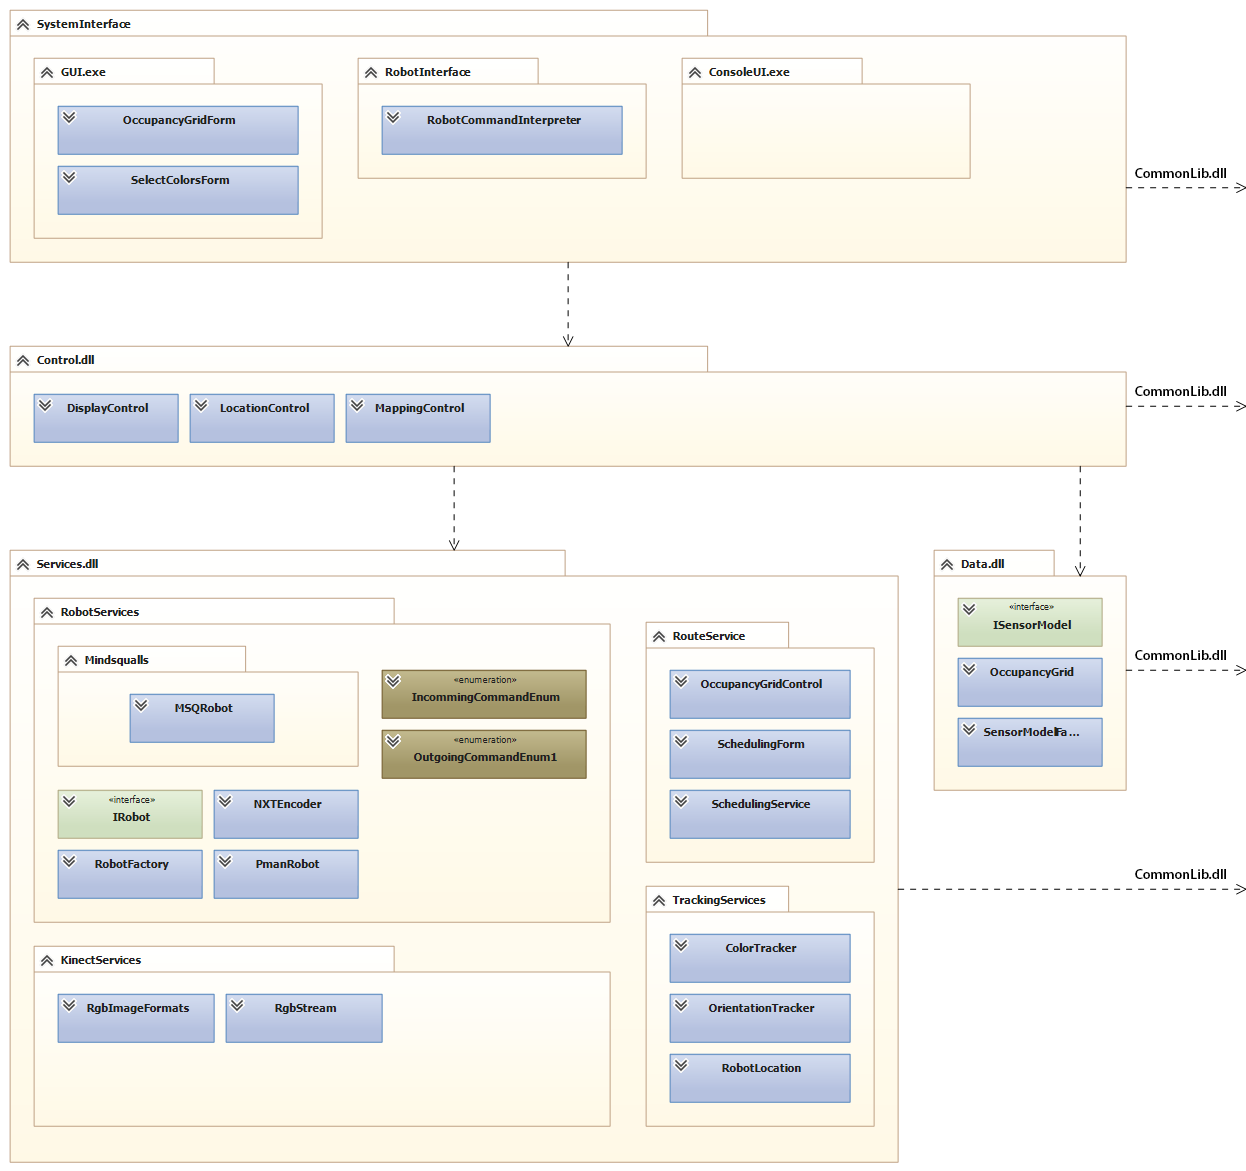
\includegraphics[width=1\textwidth]{./graphics/systemarkitektur_1}
\caption{Lagene i systemarkitekturen med deres ydre associationer. Associationerne til højre fører alle til \lstinline[style=csharp]!CommonLib.dll!, som ses på \cref{arkitektur:klassediagram:2}.}
\label{arkitektur:klassediagram:1}
\end{figure}

\begin{figure}
\centering
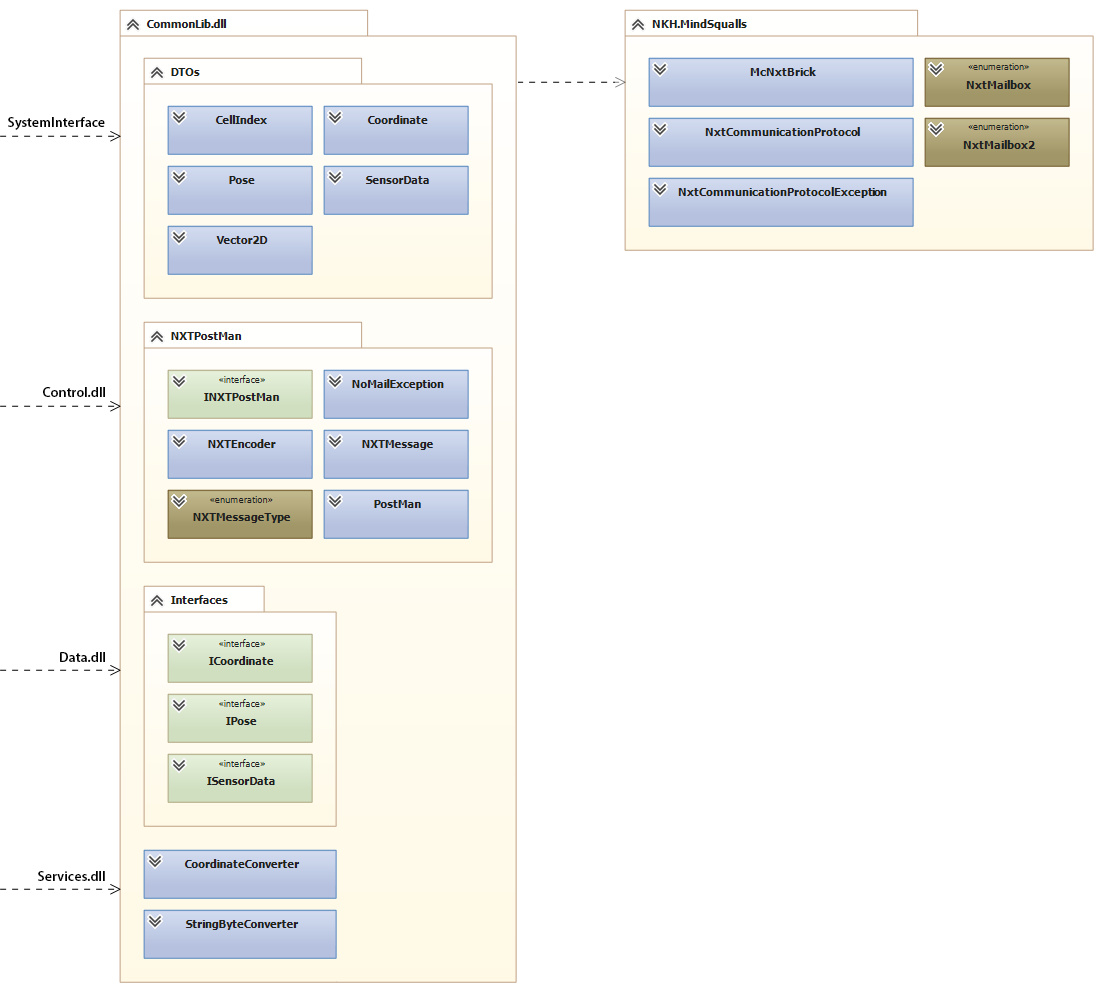
\includegraphics[width=1\textwidth]{./graphics/systemarkitektur_2}
\caption{Viser namespacet \lstinline!CommonLib.dll! (uden interne associationer), som er en del af den lagdelte systemarkitektur. De fleste lag i arkitekturen har associationer til netop \lstinline!CommonLib.dll!, der indeholder de elementer, som benyttes af alle lag. De refererende namespaces kan ses på \cref{arkitektur:klassediagram:1}.}
\label{arkitektur:klassediagram:2}
\end{figure}
\section{CommonLib.dll}\label{arkitektur:commonlib}
Benyttes af alle lag i arkitekturen.
Dets formål er at samle de komponenter som i systemet kan benyttes af alle lag.
Derfor holder det også en reference til namespacet \lstinline[style=csharp]!NKH.MindSqualls! for at kunne tilgå den del af MindSqualls (\cref{mindsqualls}) som indeholder kommunikationen til NXT-enheden.

\paragraph{CommonLib.DTOs}
Dette namespace indeholder alle \textit{Data Transferring Objects} som har til opgave at sende data mellem de forskellige lag.

\paragraph{CommonLib.NXTPostMan}
Som navnet på namespacet antyder, så er formålet med \lstinline[style=csharp]!CommonLib.NXTPostMan! at sende beskeder frem og tilbage mellem PC og robotten; hvilket gør det ansvarlig for al kommunikation imellem de to, som beskrives detaljeret i \cref{kommunikation}.

\paragraph{CommonLib.Interfaces}
Definerer en række interfaces, som implementeres af de respektive DTO'er.
Dette minimerer koblingen af koden og gør dem samtidig mere modulær, da komponenter nemt kan udskiftes.

\section{NKH.MindSqualls}\label{arkitektur:mindsqualls}
Dette er koden fra MindSqualls frameworket (beskrevet i \cref{mindsqualls}).
Det er dog ikke alle komponenter i frameworket der benyttes; det benyttes primært til at etablere kommunikation mellem NXT-enheden og PC samt exceptions, hvilket implementeres gennem \lstinline[style=csharp]|PostMan| klassen.

\section{SystemInterface}\label{arkitektur:systeminterface}
Dette er "indgangen" til systemet og er derfor også den komponent, som er ansvarlig for alle ydre påvirkninger; det være sig f.eks. brugerinput eller andre systemer, som ønsker at tilgå systemet.

\paragraph{SystemInterface.GUI.exe}
Dette namespace indeholder de grafiske komponenter for systemet, og er derfor programmet, der starter systemet.
Det er ansvarlig for at modtage og reagere på brugerens input.

\paragraph{SystemInterface.RobotInterface}
Essensen i dette namespace er en tråd, der konstant tjekker efter nye beskeder på NXT-enheden.
Den benytter så henholdsvis \lstinline[style=csharp]|LocationControl| og \lstinline[style=csharp]|MappingControl| til at reagere på beskeder den finder, og anmoder dermed \lstinline[style=csharp]!Services! namespacet om at udføre den pågældende handling.

\section{Control.dll}\label{arkitektur:control}
Denne komponent i arkitekturen er ansvarlig for kontrol af robotten samt opdatering af data.
Kald hertil stammer fra \lstinline[style=csharp]!SystemInterface!, der anmoder om en action, som dette namespace så reagerer på ved at benytte \lstinline[style=csharp]!Services! namespacet.

\paragraph{Control.DisplayControl}
Er en klasse som henter en videostrøm fra farvekameraet på en Microsoft Kinect.

\paragraph{Control.LocationControl}
Denne klasse opdaterer lokationen af robotten.
Den indeholder således også information om robottens omgivelser og robotten selv.

\paragraph{Control.MappingControl}
Al kontrol af robotten på kortet (occupancy grid) foregår gennem denne klasse.
Den indeholder således metoder til at sende robotten til et nyt koordinat, opdatere kortet og hente nye sensormålinger.

\section{Services.dll}\label{arkitektur:services}
Dette er det nederste lag i arkitekturen og benyttes af \lstinline[style=csharp]!Control! namespacet når en handling ønskes udført.

\paragraph{Services.RobotServices}
Dette namespace benyttes, når robotten skal kontrolleres.
Det er således herigennem, der sendes beskeder til robotten, for at få den til at bevæge sig til en ny position og tage sensormålinger.

\paragraph{Services.RouteService}
For at få robotten til at køre en rute på kortet benyttes \lstinline[style=csharp]!RouteService! namespacet, der består af en grafisk komponent, der gør det muligt at klikke en rute ind på et occupancy grid samt en \lstinline[style=csharp]|SchedulingService|, der returnerer en kø af de punkter, som ruten består af.

\paragraph{Services.KinectServices}
Benyttes af \lstinline[style=csharp]!Control.DisplayControl! for at vise en videostrøm fra farvekameraet i Kinecten.
Konverterer den returnerede videostrøm til en strøm af bitmaps, som kan vises grafisk i \lstinline[style=csharp]!SystemInterface!.

\paragraph{Services.TrackingServices}
Denne service er ansvarlig for at holde styr på robottens lokation samt positur.
Robotten kan således gennem \lstinline[style=csharp]!Control! benytte dette namespace, når den ønsker en opdatering af sin positur.

\section{Data.dll}\label{arkitektur:data}
Dette assembly indeholder alle data objekter for occupancy grid samt sensormodellen.
Alt data opdateres fra \lstinline[style=csharp]!Control! når robotten har taget en ny måling.






